\documentclass[pidr]{tnreport}
%\documentclass[confidential,pidr]{tnreport} % If you are writing confidential report

\usepackage{multirow}
\usepackage[]{algorithm2e}
\usepackage{float}

\def\reportTitle{Comparateur d'algorithmes de plus court chemin} % Titre du mémoire
\def\reportLongTitle{Benchmarking d'algorithmes de plus court chemins sur grilles générées aléatoirement} % Titre plus long du mémoire

\def\reportAuthor{Vincent \textsc{Albert}\\ Nicolas \textsc{Bédrine}}
\def\reportAuthorEmail{\email{vincent.albert@telecomnancy.eu}\\ \email{nicolas.bedrine@telecomnancy.eu}} % Courriel de l'élève

\def\reportSupervisor{M.~Olivier Buffet} % Prénom Nom de l'encadrant industriel

\def\reportCompany{Loria} % Nom de l'entreprise d'accueil
\def\reportCompanyAddress{615, Rue du Jardin botanique}  % Adresse de l'entreprise
\def\reportCompanyCity{54506, Vandœuvre-lès-Nancy} % Adresse (cont.) de l'entreprise
\def\reportCompanyPhone{03 83 59 20 00} % Téléphone de l'entreprise
\def\reportCompanyLogoPath{figures/loria.jpg} % Logo de l'entreprise -- comment this definition to remove company logo

\def\place{Villers-lès-Nancy} % Ville pour la signature pour l'engagement anti-plagiat
\def\date{\today} % Date pour la signature de l'engagement anti-plagiat

\def\reportProjectCustomer{Projet réalisé pour l'équipe Maia du laboratoire Loria}


\begin{document}
  
\maketitle
\pagenumbering{roman}

\insertAntiPlagiarismAgreement{\textsc{Albert}, Vincent}{1205033068}
\insertAntiPlagiarismAgreement{\textsc{Bédrine}, Nicolas}{}

\clearpage
\makesecondtitle

\section*{Remerciements}
\addcontentsline{toc}{chapter}{Remerciements}

{\em
Nous tenons à remercier toutes les personnes nous ayant accompagnés durant la réalisation de ce projet, et en particulier de M.~Buffet pour nous avoir encadré durant toute la durée du projet et pour nous avoir prodigué ses précieux conseils. \\
Nous remercions aussi M.~Jean-François \textsc{Scheid} qui a supervisé l'organisation des PIDRs et de Mme~Isabelle \textsc{Chenet}, secrétaire des PIDRs. \\
Enfin, nous remercions toute l'équipe pédagogique et administrative de TELECOM Nancy pour nous fournir un cadre d'études adéquat à la réalisation de ce projet. \\
}

\clearpage

\section*{Avant-propos}
\addcontentsline{toc}{chapter}{Avant-propos}
Ce rapport est le résultat d'un projet de découverte de la recherche de quatre mois effectué dans le cadre du sujet fourni par M.~Olivier \textsc{Buffet}, chercheur au Loria. \\
Le projet a été réalise pour l'équipe Maia (MAchines Intelligentes Autonomes), groupe de recherches centré sur les comportements décisionnels intelligents. Ses principaux champs de recherches sont les systèmes multi-agents et complexes ainsi que les systèmes décisionnels incertains. \\
N'ayant que peu d'expérience dans le domaine de l'Intelligence Artificielle mais étant très intéressé par cette dernière, nous avons choisi ce sujet afin d'en approfondir nos connaissances. Étant donné notre méconnaissance de la plupart des algorithmes de plus courts chemin, nous nous sommes demandés quelles en sont les principales différences. \\ 
Notre étude portant sur l'implémentation des algorithmes ainsi que de leurs comparaison au travers de batteries de tests était donc l'occasion d'en apprendre plus sur leur fonctionnement.

\clearpage

\renewcommand{\baselinestretch}{0.5}\normalsize
\tableofcontents
\renewcommand{\baselinestretch}{1.0}\normalsize
\clearpage

\pagenumbering{arabic}
\setcounter{page}{1}

\chapter{Introduction}

	\section{État actuel du domaine de recherches et légitimité du sujet}

\paragraph{}
Les algorithmes de plus court chemin appartiennent à la théorie des graphes et constituent un vaste champ de recherches de l'Intelligence Artificielle. Il existe de nombreux algorithmes qui ont été développés depuis les débuts de la Recherche Opérationnelle au début des années 1940, les plus connus étant Dijkstra et A*.

\paragraph{}
Cependant, bien que ces algorithmes soient connus et maîtrisés, il est difficile de déterminer \textit{a priori} leur comportement sur différents types d'environnements, et donc de savoir lequel sera le plus efficace. \linebreak

	\section{Présentation du fonctionnement global et de l'utilisation du logiciel}

\paragraph{}
Le projet se propose donc de permettre de réaliser des séquences de tests de différents algorithmes sélectionnés par l'utilisateur sur des environnements différents générés aléatoirement.

		\subsection{Fonctionnement du projet}
		
			\subsection{Les environnements}

\paragraph{}
Les environnements correspondent aux graphes sur lesquels les algorithmes sont appliqués. Il existe deux types d'algorithmes : les algorithmes générés sous forme de grilles à N dimensions avec N > 1 (hypercubes) et des environnements générés de manière totalement aléatoires.
			
			\subsection{Les algorithmes}

\paragraph{}
Plusieurs algorithmes ont été implémentés afin de tester leur efficacité sur différents types d'environnements de différentes tailles. Leur point de départ et d'arrivée sont définis aléatoirement. Les algorithmes parcourent le graphe en explorant ses noeuds par accès directs.
		
		\subsection{Lancer le projet}

\paragraph{}
Afin de répondre à tout type de besoins, le jar exécutable du logiciel prend en paramètre plusieurs options permettant différents modes d'expérimentation.

			\subsubsection{En vue graphique}

\paragraph{}
En lançant le logiciel avec la commande : \emph{java -jar AlgoComparator.jar --view}, celui-ci se lance en mode graphique. Cependant cette option a été implémentée au début du développement, avant que nous nous rendions compte qu'elle ne nous était pas utile. Elle a donc été délaissée et n'est plus fonctionnelle.

			\subsubsection{En console avec dialogue utilisateur}

\paragraph{}
En lançant le logiciel avec la commande : \emph{java -jar AlgoComparator.jar --console}, celui-ci se lance en mode console et initie un dialogue avec l'utilisateur. Il lui permettra de créer un environnement, de sauvegarder la graine, de lancer une expérience et d'enregistrer les résultats dans un fichier de logs.

			\subsubsection{En console en mode de benchmarking}
			
\paragraph{}
En lançant le logiciel avec la commande : \emph{java -jar AlgoComparator.jar --bench}, celui-ci se lance en mode benchmarking. Il va charger la configuration dans le fichier bench.conf afin de déterminer la taille et le nombre de dimensions des environnements à générer. Un seul dialogue se lance avec l'utilisateur en début d'exécution pour lui demander les algorithmes qu'il veut lancer. Tous les résultats sont stockés dans le fichier "logs.txt". \linebreak
\emph{Note: l'option --bench all permet de lancer un benchmarking sur tous les algorithmes existants et supprime la séquence de dialogue.}
			
			\subsubsection{Tester la génération d'environnements}

\paragraph{}
Etant donné que nous avons rencontré des difficultés lors de la génération des environnements durant une certaine période du développement, nous avons aussi ajouté une option permettant de lancer un benchmarking sur la création d'environnements de 10 à plusieurs millions de points. Cette option est accessible avec la commande \emph{java -jar AlgoComparator.jar --test consenv}. \linebreak
Il est aussi possible d'avoir le test de l'affichage graphique d'un environnement en remplaçant l'option \textsc{consenv} par l'option \textsc{graphenv}. Ceci peut-être pratique pour vérifier que la création des liens entre les points se fait correctement.

\clearpage

\chapter{Matériel et Méthode}

\paragraph{}
Nous allons maintenant voir les procédés mis en place pour le bon déroulement du projet et les outils développés afin de parvenir au résultat final.

	\section{Déroulement du projet}

		\subsection{Son organisation}

\paragraph{}
Afin d'avoir le meilleur suivi possible de l'avancement du projet, une réunion a été organisée avec l'encadrant toutes les deux semaines durant toute le période de développement du projet. En dehors de ces réunions, nous nous rencontrions afin de développer le projet en commun. Le reste du temps, nous avons programmé à distance grâce à l'utilitaire git.

		\subsection{Les technologies utilisées}

\paragraph{}
Le projet a été réalisé en Java sous Eclipse. \linebreak
Afin de travailler au mieux en équipe et de pouvoir gérer les versions de notre projet, nous avons utilisé le gestionnaire de version git. \linebreak
		
	\section{Outils développés pour tester les algorithmes}
	
\paragraph{}
Afin de tester les algorithmes, nous avons codé des outils nous permettant de tester l'efficacité des algorithmes que nous allons présenter ci-dessous.

		\subsection{Les environnements}

\paragraph{}
Le premier et plus important de ces outils est le générateur d'environnements permettant de tester un algorithme sous plusieurs configurations possibles.

			\subsubsection{Présentation générale de la conception des environnements : listes d'adjacence}
			
\paragraph{}
Tous les environnements sont conçus de la même façon. Ce sont des ensembles de places (représentées par N coordonnées pour N dimensions) reliées entre elles par des liens pondérés. Afin de représenter ces liens, nous possédons une liste d'adjacence associant à chacun des points la liste de ses successeurs. Chacune des dimensions possède une borne supérieure et inférieure.
	
			\subsubsection{Les environnements aléatoires}

\paragraph{}
Au début du projet, nous voulions générer aléatoirement des graphes orientés. Cependant nos premiers échecs furent infructueux ; nos graphes n'étaient en effet jamais suffisamment connexes pour qu'une solution existe. Nous avons alors recherché un moyen de générer un environnement aléatoire, orienté et fortement connexes, mais ils semblerait que cela soit encore du domaine de la recherche. Ceci n'étant pas l'axe principal de notre projet, nous avons décidé d'abandonner ce type de graphe afin de nous concentrer sur lagénération de grilles.
			
			\subsubsection{Les grilles et hypercubes}
		
\paragraph{}
Le principal type d'environnement utilisé sont donc les grilles à N dimensions. A partir des bornes données par l'utilisateur et le nombre de places appartenant à chaque dimension du graphe, les places sont générées de manière régulière sur chaque dimension. En parallèle de la création des points, chacun d'entre eux est relié à son voisin. On sait que dans un hypercube, tous les points ont pour voisins directs les points ayant exactement un coordonnées différente. A partir de là il est facile de générer le lien entre la place courante et tous les points qui ont été précédemment générés. \newline
Les liens sont pondérés pseudo-aléatoirement à partir d'un RNG alimenté par une graine spécifique (dans notre cas, le timestamp).
		
			\subsubsection{Génération d'environnement par graine : l'objet Seed}

\paragraph{}
Afin d'enregistrer facilement les données relatives à un graphe sans enregistrer la totalité des points (ce qui pourrait être une  perte considérable de place dans le cas d'un environnement à plusieurs millions de points), nous enregistrons toutes les données nécessaires à la génération d'un environnement dans un fichier texte, ce qui nous permettra par la suite de recréer exactement le même environnement sans sauvegarder tous les points. 

\paragraph{}
Les données enregistrées sont la graine (le timestamp lors de la première création de l'environnement), le nombre de points pour chacune des dimensions (nous sommes dans le cas des grilles et hypercubes) ainsi que la borne min et la borne inf des points (toutes les bornes sont considérées comme identiques, les hypercubes sont donc réguliers).

\paragraph{}
L'objet Seed de notre programme permet, à partir d'un fichier texte formaté, de reproduire à l'identique le graphe d'une environnement.

			\subsubsection{Les refactorisations du modèle des environnements}

\paragraph{}
Étant donné qu'au début nous désirions créer des environnements aléatoires, l'ensemble du code de nos Environnements se basait sur les positions des places dans le graphe. Or de cette manière, des parcours supplémentaires étaient obligatoires afin de rechercher des places par leurs coordonnées, ce qui ralentissait considérablement notre code. 
\paragraph{}
Cependant une fois les graphes aléatoires abandonnés, nous nous sommes rendus qu'il était bien plus facile et rapide de générer les graphes en grille à partir de leurs indices. Nous avons donc développé une seconde version plus efficace (étant donné que le nombre de dimensions et de points par dimension est connu à l'avance).
\paragraph{}
Cependant en effectuant des recherches, nous avons vu le principe de génération d'hypercubes de dimension N récursivement par fusion d'hypercubes de dimension N-1. Nous avons donc décidé d'adapter ce principe à nos grilles en N dimensions et à M points.

Voici les images exposant ce principe et dont nous nous sommes inspirés : 

\begin{figure}[H]
    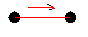
\includegraphics[width=0.15\textwidth]{./figures/Hypercube-dim1.PNG}
    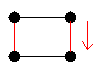
\includegraphics[width=0.15\textwidth]{./figures/Hypercube-dim2.PNG}
    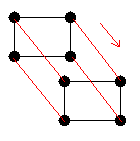
\includegraphics[width=0.2\textwidth]{./figures/Hypercube-dim3.PNG}
    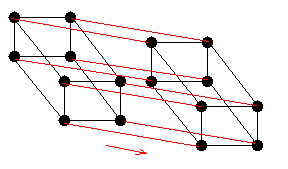
\includegraphics[width=0.4\textwidth]{./figures/Hypercube-dim4.PNG}
    \caption{Génération d'un hypercube en 4 dimensions}
\end{figure}

\paragraph{}
Nous avons donc refactorisé le code des Environnements afin d'appliquer cette modification, et la différence fut flagrante. Alors qu'il était impossible de générer un environnement d'un million de points dans la première version (même après plusieurs heures), le nouvel algorithme était capable de le faire en moins d'une dizaine de secondes. \linebreak
Voici l'algorithme que nous avons implémenté : 

\begin{algorithm}[H]
 \KwData{M : tableau qui associe à chaque dimension i son nombre de points, N : nombre de dimensions du graphe, borne\_inf : borne inférieure de toutes les dimensions, borne\_sup : borne supérieure de toutes les dimensions, i : compteur correspondant à la dimension courante, j : compteur correspondant au nombre de points de la dimension courante, graph : graph actuel que l'on fait évoluer}
 \KwResult{Hypercube de N dimensions à M[i] points chacune}

  graph = new Point(nb\_dim = N, coordonnées = \{borne\_min, ...\}) //On crée le point extremum  \linebreak
 i = 0 \linebreak
 \While{i < N}{
 //On calcule la distance entre les points de la dimension courante \linebreak
 	distance = calculerDist(M[i], borne\_inf, borne\_sup)  \linebreak
 	//On duplique le graphe le nombre de fois qu'il faut \linebreak
 	\For{j=0; j<M[i]; j++}{
 		tmp = dupliquer(graph) \linebreak
 		//On décale les coordonnées de la copie de la distance qui existe entre les points \linebreak
 		glisser\_coordonnées(tmp, distance) \linebreak
 		copies\_graph.push(tmp) \linebreak
 	}
 	graph = fusion(graph, copies\_graph) //On fusionne toutes les copies ensembles
 }
 \caption{Algorithme de génération d'une grille à N dimensions}
\end{algorithm}

\paragraph{}
Voici un tableau comparatif des différentes versions de l'algorithme de création de cartes à N dimensions :

\begin{table}[h]
\begin{center}
   \begin{tabular}{| l | r | r | r | r | r | r | r | r | r | r | r | r | r | r | r | r | r | r | r | r | r |}
     \hline
      \textbf{Version} & \multicolumn{3}{c|}{\textbf{10\up{2}}} & \multicolumn{3}{c|}{\textbf{10\up{4}}} & \multicolumn{3}{c|}{\textbf{10\up{6}}} & \multicolumn{3}{c|}{\textbf{10\up{7}}} \\
     \hline
     \cline{2-5}
    & \textbf{2D} & \textbf{3D} & \textbf{4D} & \textbf{2D} & \textbf{3D} & \textbf{4D} & \textbf{2D} & \textbf{3D} & \textbf{4D} & \textbf{2D} & \textbf{3D} & \textbf{4D}\\ \hline
     1\up{ère} version & 5 & - & - & ~10\up{7} & ~10\up{8} & ~10\up{8} & \multicolumn{3}{c|}{+$\infty$}  & \multicolumn{3}{c|}{+$\infty$}   \\ \hline
     2\up{ème} version & 2 & - & - & 34 & 36 & 41 & 16 864 & 24 247 & 32 589 & 53 789 & 74 252 & 83 736  \\ \hline
     3\up{ème} version & 2 & - & - & 13 & 16 & 23 & 368 & 512 & 746  & 14 713 & 21 697 & 37 250 \\ \hline
   \end{tabular}
 \end{center}
 \caption{Tableau récapitulatif des benchmarkings}
\end{table}

	\subsection{Les différents algorithmes implémentés}
	
		\subsection{Objet Evaluation et fichiers de log}
\paragraph{}
Le second outil nous permettant de comparer les algorithmes entre eux sont les objets Evaluation récoltant les données relatives à l'exécution de l'algorithme. Ces données sont les suivantes :

\begin{itemize}
	
	\item Le nombre de nœuds "visités" avant de trouver la première solution
	\item Le nombre total de nœuds "visités".
	\item Le nombre de nœuds "explorés".
	\item Le nombre de solutions trouvées par l'algorithme.
	\item La liste du coût pour toutes les solutions trouvées.
	\item Le nombre de nœuds appartenant au chemin de chacune des solutions.
	\item La liste du nombre de nœuds "visités" pour chaque solution.

\end{itemize}

Ce sont sur elles que se baseront les comparaisons entre les algorithmes. 		
		
		\subsection{Vue graphique}		
		
\paragraph{}
Lors de la première phase de développement, nous avons réalisé une interface graphique permettant à l'utilisateur de modifier toutes les options possibles et de lancer le déroulement d'un algorithme avec une interface graphique. Cependant cela n'était que fonctionnel pour les environnements en deux dimensions et ne correspondaient pas à nos besoins réels, nous avons donc abandonné le développement de cette fonctionnalité qui est désormais obsolète.
		

\begin{lstlisting}[language=c++, caption={Premier Exemple}, label={lst:premierExemple}]
void CEquation::IniParser()
{
	if (!pP){ //if not already initialized...
		pP = new mu::Parser;

		pP->DefineOprt("%", CEquation::Mod, 6); //deprecated
		pP->DefineFun("mod", &CEquation::Mod, false);
		pP->DefineOprt("&", AND, 1); //DEPRECATED
		pP->DefineOprt("and", AND, 1);
		pP->DefineOprt("|", OR, 1); //DEPRECATED
		pP->DefineOprt("or", OR, 1);
		pP->DefineOprt("xor", XOR, 1);
		pP->DefineInfixOprt("!", NOT);
		pP->DefineFun("floor", &CEquation::Floor, false);
		pP->DefineFun("ceil", &CEquation::Ceil, false);
		pP->DefineFun("abs", &CEquation::Abs, false);
		pP->DefineFun("rand", &CEquation::Rand, false);
		pP->DefineFun("tex", &CEquation::Tex, false);
	
		pP->DefineVar("x", &XVar);
		pP->DefineVar("y", &YVar);
		pP->DefineVar("z", &ZVar);
	}
}
\end{lstlisting}

Il est également possible d'afficher du code directement depuis un fichier source, le résultat de cette opération est visible dans le listing \ref{lst:fromSrc}
\lstinputlisting[language=c++,caption={Affichage depuis le fichier source},label={lst:fromSrc}]{figures/sourceCode.cpp}

\chapter{Résultats et interprétation}
	
	\section{Exécution des algorithmes sur les environnements}
		
		\subsection{Présentation des résultats et comparaison}
		
		\subsection{Interprétation des résultats}

\chapter{Discussion globale}

\clearpage
\renewcommand{\tocbibname}{Bibliographie / Webographie}
\bibliography{example} % See example.bib 
\bibliographystyle{plain}

\clearpage

\listoffigures
\clearpage

\listoftables
\clearpage

\lstlistoflistings
\clearpage

\chapter*{Glossaire}
\addcontentsline{toc}{chapter}{Glossaire}

\clearpage
\renewcommand{\thesubsection}{\Roman{subsection}}

\appendix
\part*{Annexes}
\addcontentsline{toc}{part}{Annexes}
\clearpage

\chapter{Première Annexe}
\clearpage

\chapter{Seconde Annexe}


\clearpage
\thispagestyle{empty}

\section*{Résumé}
\addcontentsline{toc}{chapter}{Résumé}

\paragraph{Le sujet en bref.}
Le sujet qui a été choisi porte sur la réalisation d'un logiciel de benchmarking permettant de tester et de comparer différents algorithmes de recherche de plus court chemin sur des environnements diversifiés générés aléatoirement sur des séquences de tests paramétrées dans un fichier de configuration. \linebreak

\paragraph{Les fonctionnalités implémentées.}

\paragraph{Les résultats.}

\paragraph{Interprétation.}

{\bf Mots-clés :} algorithmes de plus court chemin, théorie des graphes, environnements aléatoires, benchmarking, interface utilisateur, graines.

\end{document}